\documentclass[11pt, oneside]{article} 
\usepackage{geometry}
\geometry{letterpaper} 
\usepackage{graphicx}
	
\usepackage{amssymb}
\usepackage{amsmath}
\usepackage{parskip}
\usepackage{color}
\usepackage{hyperref}

\graphicspath{{/Users/telliott/Github/calculus_book/png/}}
% \begin{center} 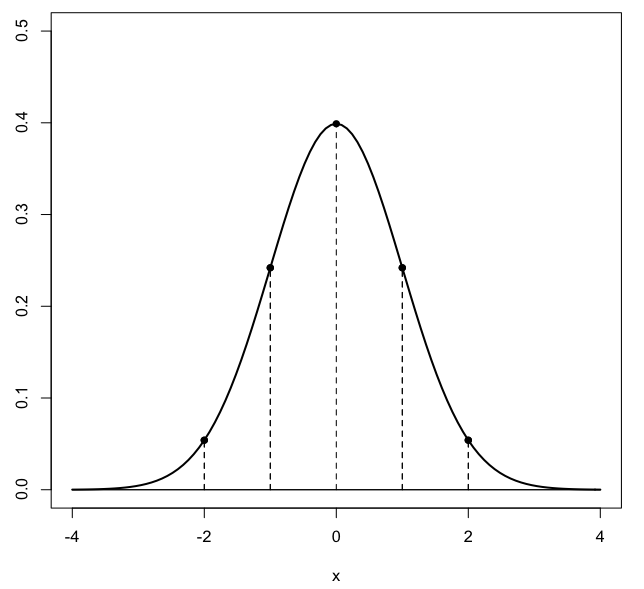
\includegraphics [scale=0.4] {gauss3.png} \end{center}

\title{Circles and ellipses}
\date{}

\begin{document}
\maketitle
\Large

A circle can be defined as all the points at the same distance from a central point, let us label that point $(h,k)$.  The distance from the points to the center is the radius, denoted $r$.

Using the Pythagorean theorem, we can calculate the square of the distance from the origin as
\[ r^2 = (x - h)^2 + (y - k)^2 \]

The simplest circles are those whose central point is the origin of the coordinate system.  In that case the equation  simplifies to 
\[ r^2 = x^2 + y^2 \]
Usually, we know the value of $r$ and we want to write an equation for $y$ in terms of $x$.  Then
\[ y^2 = r^2 - x^2 \]
\[ y = \sqrt{r^2 - x^2} \]

\subsection*{tangent to the circle}

Suppose we have a unit circle and an external point $(x,y)$.  We wish to find the equation of the tangent line to a point on the circle.  Call that point $(a,b)$.

Circles are special.  Any tangent is perpendicular to the radius at the point of tangency.  

The line through $(a,b)$ and the origin has slope $b/a$ since
\[ m = \frac{b - 0}{a - 0} \]

If we have two lines with slopes $m_1$ and $m_2$ and they are perpendicular, the product is $-1$.  So the tangent to the circle at $(a,b)$ has slope $-a/b$ and the line through $(x,y)$ and $(a,b)$ is

\[ -\frac{a}{b} = \frac{y - b}{x - a} \]
\[ - ax + a^2 = by - b^2 \]

We also have that $a^2 + b^2 = 1$ so
\[ ax + by = 1 \]

which is a long-winded way of arriving at what we had above, a line with slope $-a/b$ whose $y$-intercept is $0$.

Substitute into the equation of the circle:
\[ a^2 + (\frac{1 - ax}{y})^2 = 1 \]
\[ a^2y + 1 - 2ax + a^2x^2 = y \]
\[ (y + x^2)a^2 - 2xa + (1 - y) = 0 \]

We have a quadratic in $a$.  For a particular $x$ and $y$, we can solve for $a$ and then $b$.

\subsection*{ellipse}
I found a problem on the web that extends this to the ellipse:

\url{https://math.stackexchange.com/questions/834392/equations-of-lines-tangent-to-an-ellipse}

In working that problem, I ended up with a quartic equation (fourth power).  This is, quite literally, a mess.

Here's a great idea for ellipse problems:  Stretch and rescale the problem to one involving a circle, by using a \emph{change of variable}.  Suppose the ellipse is
\[ \frac{x^2}{a^2} + \frac{y^2}{b^2} = 1 \]
Let $x = au$ and $y = bv$.  Then
\[ \frac{a^2u^2}{a^2} + \frac{b^2 v^2}{b^2} = 1 \]
\[ u^2 + v^2 = 1 \]

The ellipse has become a unit circle!

Apply the same transformation to any points in the problem, solve the problem, and then reverse the transformation.


\end{document}